\chapter{Regression Model-based Features}
\label{sec:regressionmodels}

Semi-physical behavior about a building can be extracted by using performance prediction models and using output parameters and goodness-of-fit metrics for characterization. This section covers the use of several common electrical consumption prediction models to create sets of temporal features useful for characterization of buildings. Section \ref{sec:modelbasedtheory} covers the theory underlying each technique and Section \ref{sec:modelbaseddiscussion} discusses the implementation of the case study data with a focus on underlying trends as related to building use type.

\section{Theoretical Basis}
\label{sec:modelbasedtheory}
\subsection{Load shape regression-based Features}
\label{sec:regressionmetrics}

Prediction of electrical loads based on their shape and trends over time is a mature field developed to forecast consumption to detect anomalies and analyze the impact of demand response and efficiency measures. The most common technique in this category is the use of heating and cooling degree days to normalize monthly consumption \citep{fels_prism:_1986}. Over the years, various other techniques have been developed using techniques such as neural networks, ARIMA models, and more complex regression \citep{taylor_comparison_2006}. However, simplified methods have retained their usefulness over time due to ease of implementation and accuracy. In the context of temporal feature creation, a regression model provides various metrics that describe how well a meter conforms to conventional assumptions. For example, if actual measurements and predicted consumption match well, the underlying behavior of energy-consuming systems in the building has been captured adequately. If not, there is the uncharacterized phenomenon that will need to be obtained with a different type of model or feature. 

A contemporary, simplified load prediction technique is selected to create temporal features that capture whether the electrical measurement is simply a function of time-of-week scheduling. This model was developed by Matthieu et al. and Price and implemented mostly in the context of electrical demand response evaluation \citep{price_methods_2010, mathieu_quantifying_2011}. The premise of the model is based on two features: a time-of-week indicator and an outdoor air temperature dependence. This model is also known as the \emph{Time-of-week and Temperature or (TOWT)} model or \emph{LBNL regression model} and is implemented in the \emph{eetd-loadshape} library developed by Lawrence Berkeley National Laboratory\footnote{https://bitbucket.org/berkeleylab/eetd-loadshape}.

According to the literature, the model operates as follows \citep{price_methods_2010}. The time of week indicator is created by dividing each week into a set of intervals corresponding to each hour of the week. For example, the first interval is Sunday at 01:00, the second is Sunday at 02:00, and so on. The last, or 168th, interval is Saturday at 23:00. A different regression coefficient, $\alpha_i$, is calculated for each interval in addition to temperature dependence. The model uses outdoor air temperature dependence to divide the intervals into two categories: one for occupied hours and one for unoccupied. These modes are not necessarily indicators of exactly when people are inhabiting the building, but simply an empirical indication of when occupancy-related systems are detected to be operating. Separate piecewise-continuous temperature dependencies are then calculated for each type of mode. The outdoor air temperature is divided into six equally sized temperature intervals. A temperature parameter, $\beta_j$, with $j = 1...6$, is assigned to each interval. Within the model, the outdoor air temperature at time, $t$, occurring at time-of-week, $i$, (designated as $T(t_i)$) is divided into six component temperatures, $T_{c,j}(t_i)$. Each of these temperatures is multiplied by $\beta_j$ and then summed to determine the temperature-dependent load. For occupied periods the building load, $L_o$, is calculated by Equation \ref{eq:tempdepload}.

\begin{equation}
\label{eq:tempdepload}
L_0(t_i,T(t_i) = \alpha_i + \sum_{j=1}^{6}\beta_j T_{c,j}(t_i)
\end{equation}

Prediction of unoccupied mode occurs using a single temperature parameter, $\beta_u$. Unnoccupied load, $L_u$, is calculated with Equation \ref{eq:nontempdepload}.

\begin{equation}
\label{eq:nontempdepload}
L_0(t_i,T(t_i) = \alpha_i + \beta_u T_{c,j}(t_i)
\end{equation}

The primary means of temporal feature creation from this process is through the analysis of model fit. The first metric calculated is a normalized, hourly residual, $R$, that can be used to visualize deviations from the model. It is calculated from the actual load, $L_a$, and the predicted load, $L_p$. The residual at a specific hour, $t$, is calculated using Equation \ref{eq:residualerror}.

\begin{equation}
\label{eq:residualerror}
R_t = \frac{L_{t,a} - L_{t,p}}{max_{L_a}}
\end{equation}

An example of the TOWT model implemented on one of the case study buildings is seen in Figure \ref{fig:loadshape_single}. Two primary characteristics are captured from a model residual analysis. The first is the building's primary deviation from a set time-of-week schedule and behavior causing the model to highly over-predict. These deviations are most often attributed to public holidays, breaks in normal operation, or changes in normal operating modes. In the single building study, one of the most obvious daily deviations, Christmas Day, is observed. This day is significantly over-predicted due to the model not being informed of the Christmas Day holiday. The automated capture of this phenomenon can inform whether the building is of a certain use-type or in a certain jurisdiction. The second characteristic captured are periods of under prediction when the building is consuming more electricity than expected. These data inform whether a building is being consistently utilized, or whether there is volatility in its normal operating schedule from week-to-week. 

\begin{figure}[ht!]
\begin{center}
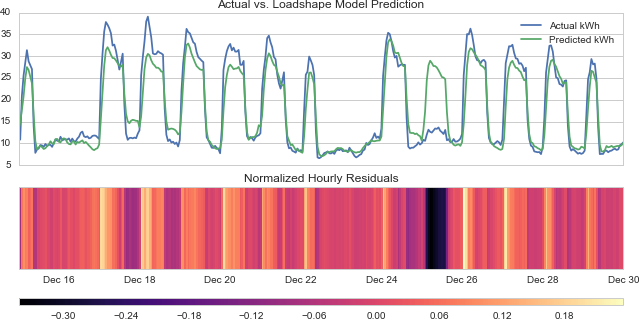
\includegraphics[width=1\columnwidth]{figures/loadshape_example/loadshape_example}
\caption{Single building example of TWOT model with hourly normalized residuals
\label{fig:loadshape_single}%
}
\end{center}
\end{figure}

\subsection{Change Point Model Regression}
\label{sec:changepointmodels}

Another means of performance modeling that takes weather characterization into consideration is the use of linear change point models. The outputs of these models can be interpretable in approximating the amount of energy being used for heating, ventilation, and air-conditioning (HvAC). This type of model has its basis in the previously-mentioned PRISM method and has been continuously utilized, recently by Kissock and Eger \citep{Kelly_Kissock_2008}. This multivariate, piece-wise regression model is developed using daily consumption and outdoor air dry-bulb temperature information. A linear regression model is fitted to data detected to be correlated with outdoor dry-bulb air temperature, either positively for cooling energy consumption or negatively for heating energy consumption. For example, as the outdoor air temperature climbs above a certain point, the relationship between electrical consumption and every degree increase in temperature should be a linear line with a certain slope if the building has an electrically-driven cooling system. The point at which this change occurs is considered the cooling balance point of the building and the slope of the line is the rate of cooling energy increase due to outdoor air conditions. This example can be seen in Figure \ref{fig:changepointmodels}a in which the base load of the building is designated as $\beta_1$, the slope of the cooling energy line is $\beta_2$, and the change point temperature is $\beta_3$. Heating energy, as seen in Figure \ref{fig:changepointmodels}b, is similar except that the slope of the line will be negative; as temperature decreases, the heating energy increases. An optimization algorithm is used to detect each of these parameters from either hourly or daily raw data.

\begin{figure}[ht!]
\begin{center}
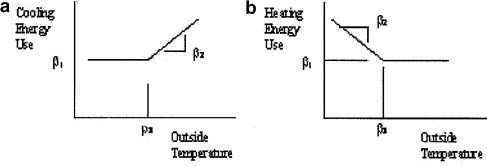
\includegraphics[width=0.84\columnwidth]{figures/changepointmodel_kissock/changepointmodel_kissock}
\caption{Example of an (a) 3 point cooling and (b) 3 point heating change point models (Used with permission from \citep{kelly_kissock_measuring_2008})
\label{fig:changepointmodels}%
}
\end{center}
\end{figure}

Equations \ref{eq:coolingenergy} and \ref{eq:heatingenergy} are used to predict energy energy consumption based on an outdoor air temperature, $T$. This equation can also predict the heating ($\beta_2(T - \beta_3)$) or cooling ($\beta_2(\beta_3 - T)$) components of the electrical consumption to a certain level of accuracy. 

\begin{equation}
\label{eq:coolingenergy}
E_c = \beta_1 + \beta_2(T - \beta_3)
\end{equation}

\begin{equation}
\label{eq:heatingenergy}
E_h = \beta_1 + \beta_2(\beta_3 - T)
\end{equation}

Figure \ref{fig:changepoint} illustrates a change point model fit on an office building in a continental climate that includes both heating and cooling seasons. It should be noted that the model is not perfectly characterizing the data due to two modes of daily operation; this situation is due to there being an offset between occupied and unoccupied operation. This model is used to generate features of approximate heating and cooling energy and in general, the slopes of these two modes can safely be assumed to be similar in most cases. The Open Meter Python library is used to regress these models for each building in this study \footnote{http://www.openeemeter.org/}.

\begin{figure}[ht!]
\begin{center}
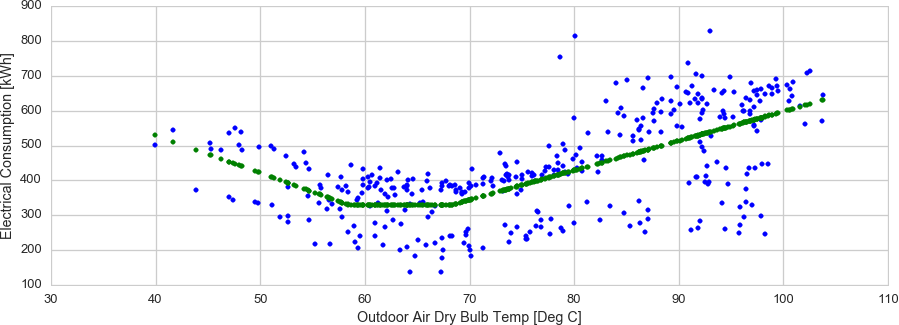
\includegraphics[width=1\columnwidth]{figures/Changepointmodelexample/Changepointmodelexample}
\caption{Single building example of change point model of a building
\label{fig:changepoint}%
}
\end{center}
\end{figure}

Figures \ref{fig:cooling_single} and \ref{fig:heating_single} illustrate single building examples of using the regression model to extract the approximate heating and cooling electrical consumption from the overall power meter. The cooling consumption example illustrates cooling consumption primarily in the summer-time season, as expected. An interesting aspect of this example is that there are a couple days of predicted cooling consumption in November and December. These days are due to outdoor air temperature crossing the balance point in anomalous ways during that season. The heating consumption example also resembles an intuitive understanding how the heating season from December to mid-April. In each example, one notices a correlation between the cooling and heating consumption in the heat-map and slight increases in the line charts indicating seasonality. 

\begin{figure}[ht!]
\begin{center}
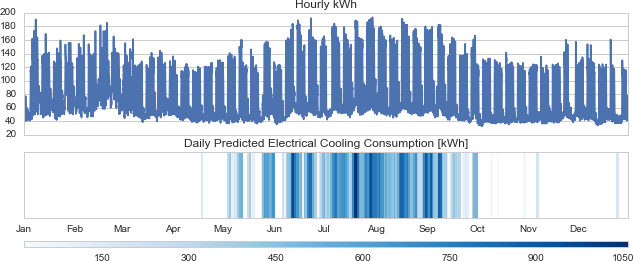
\includegraphics[width=1\columnwidth]{figures/cooling_example/cooling_example}
\caption{Single building example of predicted electrical cooling energy using change point model
\label{fig:cooling_single}%
}
\end{center}
\end{figure}

\begin{figure}[ht!]
\begin{center}
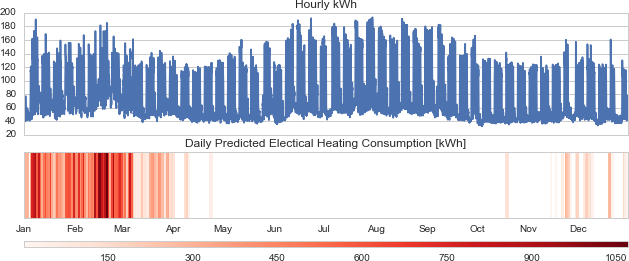
\includegraphics[width=1\columnwidth]{figures/heating_example/heating_example}
\caption{Single building example of predicted electrical heating energy using change point model
\label{fig:heating_single}%
}
\end{center}
\end{figure}

\subsection{Seasonality and Trend Decomposition}
\label{sec:seasonaldecomposition}

Temporal, or time series data, from different sources, often exhibit similar types of behavior that are studied within the field of forecasting and temporal data mining. Electrical building meter data fits within this category, and the same feature extraction techniques can be applied as what is commonly done for financial or social science analysis. These techniques often seek to decompose time-series data into several components that represent the underlying nature of the data \citep{Mitsa_2010}. For example, the electrical meter data collected from buildings is often cyclical in its weekly schedule. People are utilizing buildings each day of the week in a relatively predictable pattern. A very common example of this behavior is found in office buildings where occupants are typical white collar professionals who come into work on weekdays at a particular time and leave to go home at a certain time. Weekends are unoccupied periods in which there is little to no activity. This behavior is an example of what's known as seasonality within time series analysis. Seasonality is a fixed and known period of consistent modulation and is a feature that is often extracted before creating predictive models. 

Trends are another feature commonly found in temporal data. A trend is a long-term increase or decrease in the data that often doesn't follow a particular pattern. Trends are commonly due to factors that are less systematic than seasonality and are often due to external influences. For building energy consumption, trends manifest themselves as gradual shifts in consumption over the course of week or months. Often these shifts are due to weather-related factors having an influence on the HVAC equipment. Other causes of trends are changes in occupancy of degradation of system efficiency. 

To capture these features to understand their impact on characterizing buildings, the seasonal-trend decomposition procedure based on loess is used to extract each of these features from the case study buildings \citep{cleveland1990stl}. This process is used to remove the weekly \emph{seasonal} patterns from each building, the long-term trend over time, and the residual remainders from the model developed by those two components. The input data is aggregated to daily summations and weather normalized by subtracting the calculated heating and cooling elements from the change point model described in Section \ref{sec:changepointmodels}. This step is done to reduce the influence weather plays in the trend decomposition. The \emph{STL} package in R is used for this process to extract the seasonal, trend, and irregular components \footnote{https://stat.ethz.ch/R-manual/R-devel/library/stats/html/stl.html}. 

The details of the inner algorithms of the \emph{STL} procedure are described by Cleveland et al. \citep{cleveland1990stl}. The process uses an inner loop of algorithms to detrend and deseasonalize the data by creating a trend component, $T_v$, and a seasonal component, $S_v$. The remainder component, $R_v$, is a subtraction of the input values, $Y_v$ as seen in Equation \ref{eq:stl_residualscalc}.

\begin{equation}
\label{eq:stl_residualscalc}
R_v = Y_v - T_v - S_v
\end{equation}

 An output of the process of the \emph{STL} package is seen in Figure \ref{fig:stl_decomposition}. The \emph{data} component is the weather-normalized electrical meter data, the \emph{seasonal} component is decomposed weekly pattern, the \emph{trend} is the smoothed trend component, and the \emph{remainder} is the residual after the other components have been subtracted out.


\begin{figure}[ht!]
\begin{center}
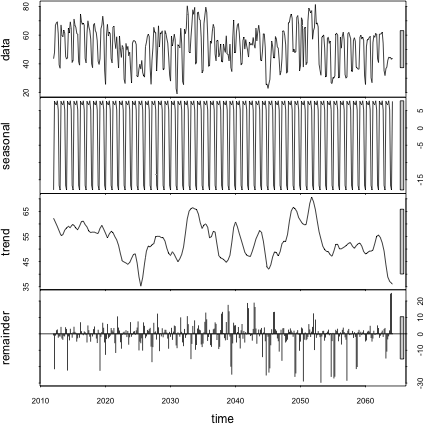
\includegraphics[width=0.7\columnwidth]{figures/stl_explanation/stl_explanation}
\caption{Output of seasonal decomposition process using loess for a single building.
\label{fig:stl_decomposition}%
}
\end{center}
\end{figure}

The seasonal component of this decomposition process can then be extracted to get an understanding of the typical weekly pattern of a building's electrical consumption. Figure \ref{fig:weeklypattern_single} illustrates this situation for a single building that has a typical office-style utilization schedule with a Monday to Friday working schedule with Saturday and Sunday off. This metric has been normalized to make it comparable to other buildings.

\begin{figure}[ht!]
\begin{center}
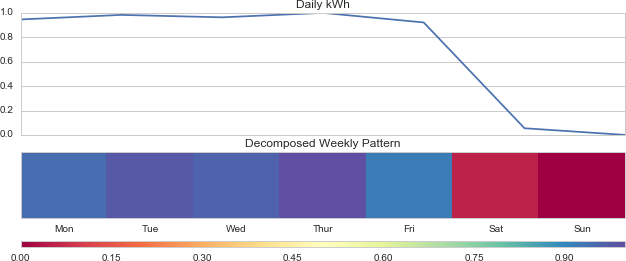
\includegraphics[width=1\columnwidth]{figures/stl_seasonal_example/stl_seasonal_example}
\caption{Single building example of decomposed weekly patterns using the \emph{STL} process
\label{fig:weeklypattern_single}%
}
\end{center}
\end{figure}


The general trend over the course of the year of data is another example of quantifying the seasonal patterns in utilization of a building. Weather influence has been reduced or removed using the change point models. Therefore, a trend could be the result of changes in building occupancy due to breaks, changes in equipment or space functions that would significantly increase or decrease the consumption, or gradual faults in systems of equipment. Figure \ref{fig:trend_single} illustrates a single building example of a decomposed trend for a building. January to May is in the middle range of consumption trend with a noticeable dip in April. From June to Oct, there is a trend upwards of higher than normal consumption, perhaps due to higher utilization of the space. October to the end of the year is back to average with a slight dip during the last few weeks of the year.

\begin{figure}[ht!]
\begin{center}
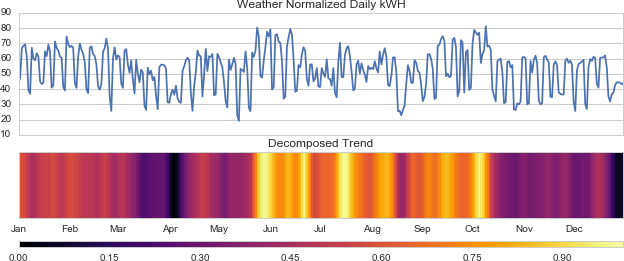
\includegraphics[width=1\columnwidth]{figures/stl_weathernorm_trend_example/stl_weathernorm_trend_example}
\caption{Single building example of decomposed trend using the \emph{STL} process
\label{fig:trend_single}%
}
\end{center}
\end{figure}


The remainder values of the \emph{STL} decomposition process are indicators of days that fall outside of the \emph{STL} model's prediction. This situation is similar to the residuals of the \emph{loadshape} models in Section \ref{sec:regressionmetrics}. Figure \ref{fig:remainder_single} illustrates an example of the residual days. Once again, this metric is normalized, however not on a 0 to 1 range. Instead, negative values indicate a lower than expected consumption for the day, while positive values are higher than average. In this example, the residuals aren't exceptionally systematic. However, a few identifiable days can be seen including Thanksgiving in November.

\begin{figure}[ht!]
\begin{center}
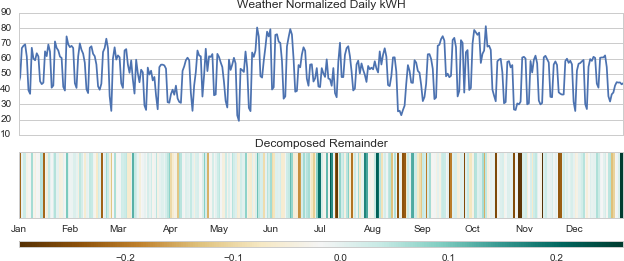
\includegraphics[width=1\columnwidth]{figures/stl_weathernorm_remainder_example/stl_weathernorm_remainder_example}
\caption{Single building example of decomposed remainder component using the \emph{STL} process
\label{fig:remainder_single}%
}
\end{center}
\end{figure}


\section{Implementation and Discussion}
\label{sec:modelbaseddiscussion}
Based on the theoretical basis of model-based approaches, the techniques are then applied to the 507 targeted case study buildings. This process enables the analysis of various patterns and phenomenon occurring in the data as a result of the building use type. Figure \ref{fig:loadshape_all} illustrates an overview of an implementation of the loadshape model on all the buildings across the various building use types in the study. The differences between each use type can be noticed from a high level due to the nature of residuals. The darker areas of the visualization indicate when the model is highly over-predicting consumption and lighter areas indicate when the model is under-predicting. Common holiday periods such as spring, summer and winter breaks and holidays such as the American Labor Day and Thanksgiving are seen as darker areas. Offices, labs and classrooms seem to have similar residual patterns, likely due to their scheduling being similar. Slight key differences are seen such as the fact that classrooms have more general areas of over-prediction, likely due to less consistent occupancy. Primary/Secondary schools and dormitories are clearly less predictable on an annual basis due to their strong seasonal patterns of use; this fact is intuitive and model residuals of this type are accurate in automatically characterizing this behavior.

\begin{figure}[ht!]
\begin{center}
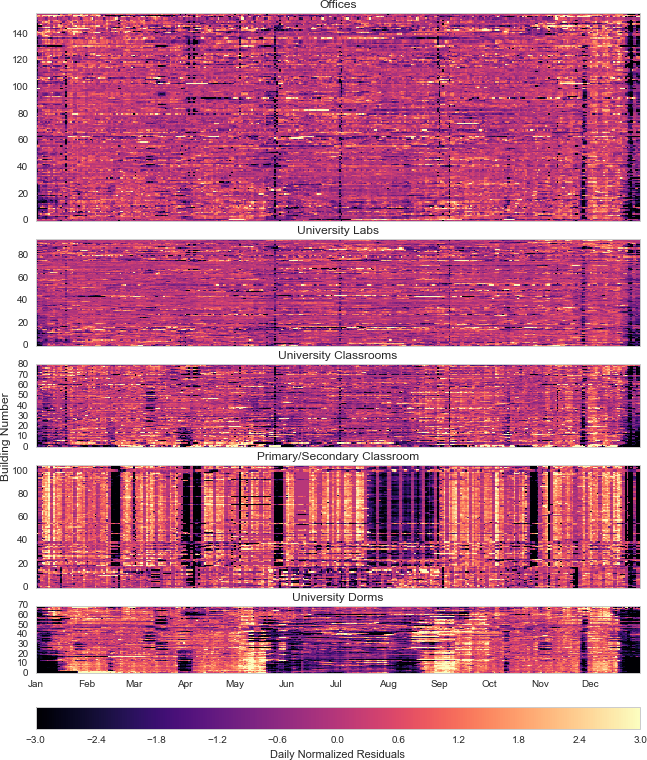
\includegraphics[width=1\columnwidth]{figures/loadshape_heatmap/loadshape_heatmap}
\caption{Heatmap of normalized daily residuals for all case study building
\label{fig:loadshape_all}%
}
\end{center}
\end{figure}

Figures \ref{fig:cooling_heatmap} and \ref{fig:heating_heatmap} illustrate heating and cooling energy regression for all case study buildings. These figures have been normalized according to floor area. Each building's response to outdoor air temperature is indicative of the type of systems installed in addition to the efficiency of energy conversion of those systems. Approximately 15-20\% of offices, labs, and classrooms have a certain amount of cooling electrical consumption, while the rest have little to none. Many of those buildings are on district heating and cooling systems, therefore, weather dependent electrical consumption is likely due to air distribution systems or auxiliary pumps. Several of the labs have year-round cooling consumption, likely due to climate and the high internal loads that accompany laboratory environments.

\begin{figure}[ht!]
\begin{center}
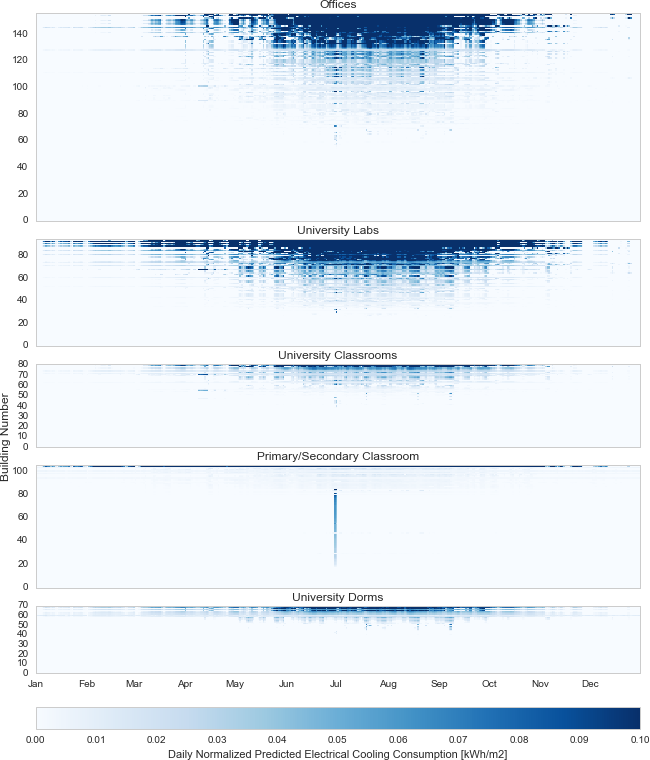
\includegraphics[width=1\columnwidth]{figures/cooling_heatmap/cooling_heatmap}
\caption{Heatmap of normalized predicted electrical cooling energy for all case study buildings
\label{fig:cooling_heatmap}%
}
\end{center}
\end{figure}

\begin{figure}[ht!]
\begin{center}
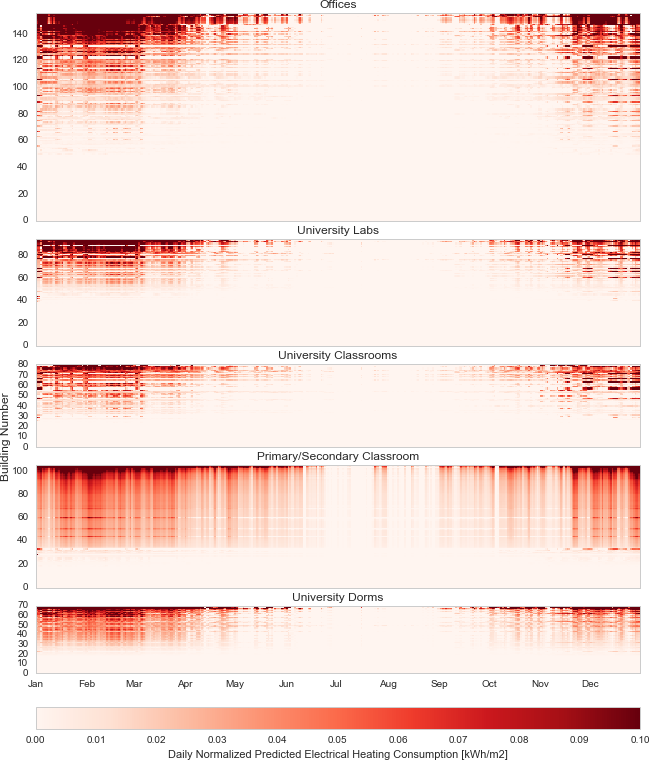
\includegraphics[width=1\columnwidth]{figures/heating_heatmap/heating_heatmap}
\caption{Heatmap of normalized predicted electrical heating energy for all case study buildings
\label{fig:heating_heatmap}%
}
\end{center}
\end{figure}


Figure \ref{fig:weeklypattern_heatmap} illustrates the weekly pattern decomposition for all of the case study buildings. For offices, most of the other cases also exhibit a typical Monday to Friday schedule, with a few exceptions that have various weekday differences and several that have higher values on Saturday. Tuesday seems to be the most consistent across the range of buildings on the peak day of consumption. University labs and classrooms appear to have the same amount of diversity and a similar schedule to offices, perhaps with slightly less use of Fridays. Primary/Secondary school classrooms appear to be the most consistent in their weekly Monday to Friday schedule and have an entirely consistent lack of Saturday and Sunday utilization. University dormitories are the most diverse in their weekly patterns with approximately half of the buildings having dominant weekday schedules and half having dominant weekend schedules.

\begin{figure}[ht!]
\begin{center}
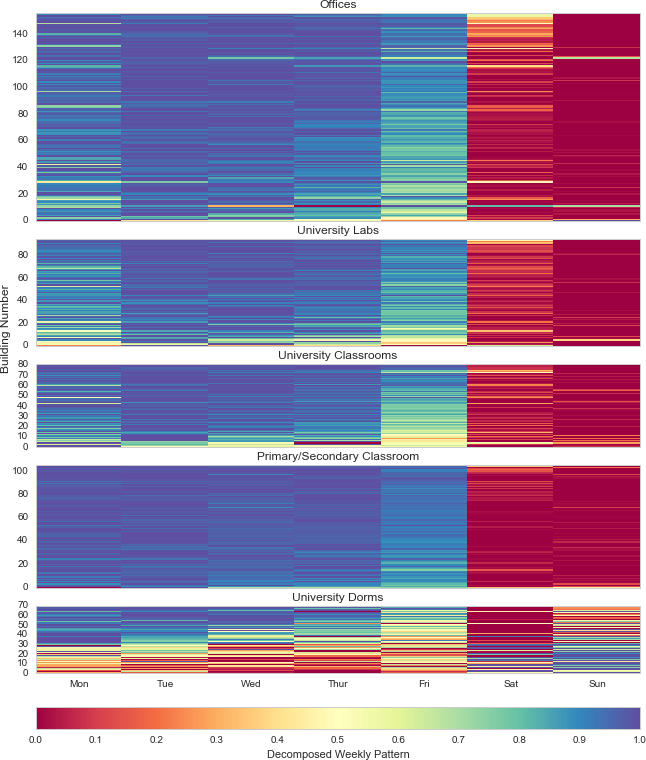
\includegraphics[width=1\columnwidth]{figures/stl_weathernorm_weeklypattern_heatmap/stl_weathernorm_weeklypattern_heatmap}
\caption{Heatmap of decomposed weekly patterns for all case study buildings
\label{fig:weeklypattern_heatmap}%
}
\end{center}
\end{figure}


Figure \ref{fig:trend_heatmap} illustrates the trend decomposition as applied to the entire case study set of buildings. Offices appear to have quite a bit of diversity over time, with a few observable systematic low spots in the spring and autumn periods at the bottom of the heat map. Laboratories reflect that behavior, while university visually has an opposite effect with lower than the average trend in the summer months. Primary/Secondary school classrooms have a very distinct delineation between when school is in session and out of session during the summer and various breaks. As many of these schools are in the UK, their out-of-session periods appear to line up naturally. University dormitories also have clear delineations between occupied and unoccupied periods and they seem also to match up quite well, despite the diversity of data sources of these buildings.

\begin{figure}[ht!]
\begin{center}
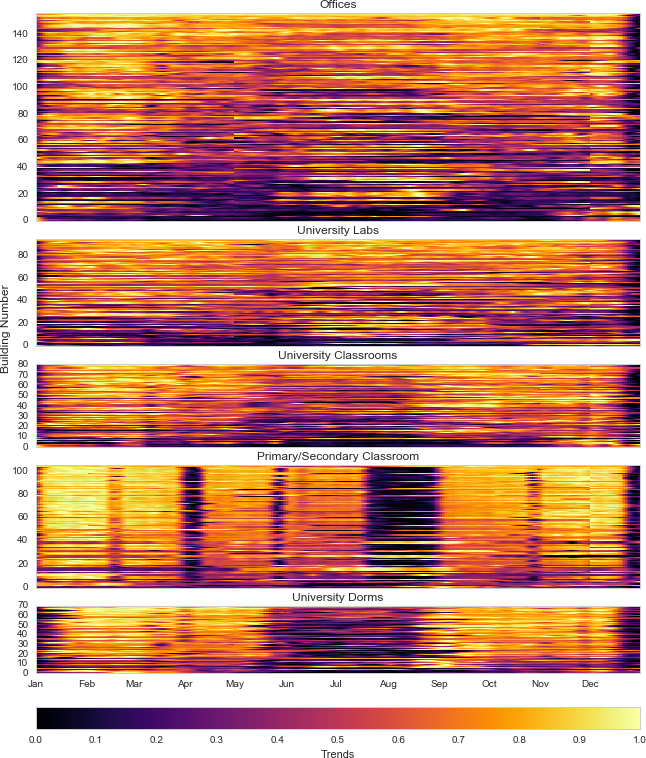
\includegraphics[width=1\columnwidth]{figures/stl_weathernorm_trend_heatmap/stl_weathernorm_trend_heatmap}
\caption{Heatmap of decomposed trend over time for all case study buildings
\label{fig:trend_heatmap}%
}
\end{center}
\end{figure}

Figure \ref{fig:residuals_heatmap} illustrates the residuals applied across all of the case study buildings. Some similarity between all of the university offices, labs, and classrooms are apparent regarding the holidays detected. The most consistent ones include the American memorial day in May, American Independence Day in July, Thanksgiving in November and Christmas Day in December. However, University Labs have a slightly less dramatic range of values. Primary/Secondary schools have appeared to have many more dramatic differences from the \emph{STL} model. 

\begin{figure}[ht!]
\begin{center}
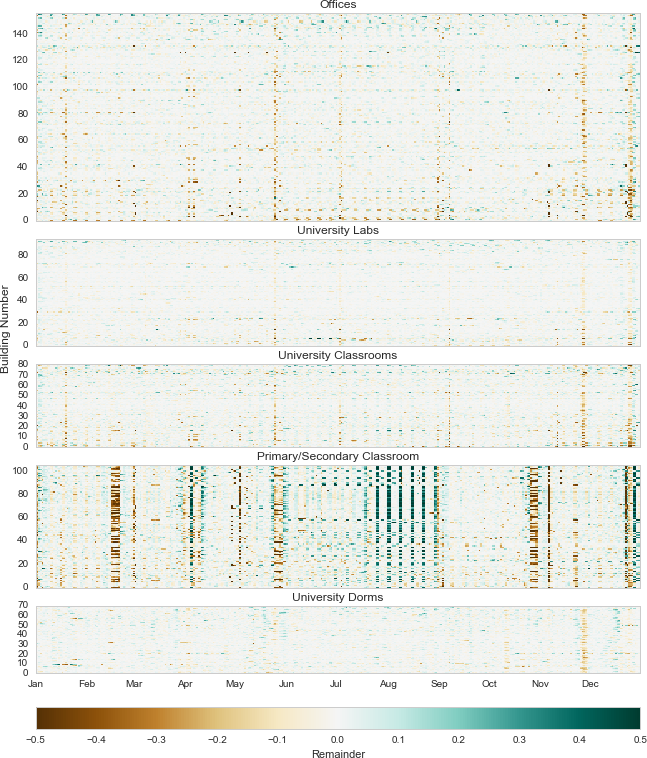
\includegraphics[width=1\columnwidth]{figures/stl_weathernorm_remainder_heatmap/stl_weathernorm_remainder_heatmap}
\caption{Heatmap of decomposed remainder residuals for all case study buildings
\label{fig:residuals_heatmap}%
}
\end{center}
\end{figure}

Overall, model-based temporal features are good at highlighting several different phenomena occurring in a building's behavior. The first, and most important, is essentially how \emph{predictable} a building is across an annual time range and what systematically anomalous days are occurring, such as holidays and break periods. Weather-related models are helpful in understanding what consumption is likely due to heating and cooling systems. This feature is different than the spearman coefficient from the statistic-based section in that it provides more information related to \emph{when} a building goes into climate control modes regarding outside air temperature.